% =================================================================
% PHYS 421: Parallel Computing — Assignment #1 report
% Filled with the student's benchmark results (WSL, GCC, OpenBLAS, NumPy)
% =================================================================

\documentclass[11pt,a4paper]{article}

% ---------- Encoding, fonts, language ----------
\usepackage[T1]{fontenc}
\usepackage[utf8]{inputenc}
\usepackage{lmodern}
\usepackage[english]{babel}

% ---------- Geometry & spacing ----------
\usepackage[a4paper,margin=1in]{geometry}
\usepackage{setspace}
\onehalfspacing
\usepackage{parskip}

% ---------- Math & symbols ----------
\usepackage{amsmath,amssymb,amsthm}
\usepackage{siunitx}
\sisetup{detect-all=true}

% ---------- Tables & graphics ----------
\usepackage{graphicx}
\usepackage{booktabs}
\usepackage{xcolor}
\usepackage{float}
\usepackage{subcaption}
\usepackage{hologo}

% ---------- Hyperlinks ----------
\usepackage[colorlinks=true,urlcolor=blue,bookmarks=true,citecolor=magenta,breaklinks=true,pdftex]{hyperref}

% ---------- Code listings ----------
\usepackage{listings}
\lstdefinestyle{pcstyle}{
	basicstyle=\ttfamily\footnotesize,
	numberstyle=\tiny, numbers=left, numbersep=8pt,
	showstringspaces=false, breaklines=true,
	frame=single, rulecolor=\color{black!20},
	keywordstyle=\color{blue!90!black},
	commentstyle=\color{green!65!black},
	stringstyle=\color{orange!80!black},
	tabsize=2, captionpos=b
}
\lstset{style=pcstyle}

% ---------- Optional PGF/TiKZ bits from template ----------
\usepackage{pgfplots}
\pgfplotsset{compat=1.18}

% ---------- Bibliography (guarded so it compiles without a .bib) ----------
\usepackage{etoolbox}
\usepackage[backend=biber,style=numeric-comp,sorting=none,sortcites=true]{biblatex}
\IfFileExists{references.bib}{\addbibresource{references.bib}}{}

% ---------- Custom metadata ----------
\newcommand{\assignmentnumber}{1}
\newcommand{\assignmenttitle}{Matrix–Matrix Multiplication: Performance and Scaling}
\newcommand{\studentname}{Adilet Akimshe}
\newcommand{\studentid}{202194337}
\newcommand{\coursecode}{PHYS 421}
\newcommand{\coursename}{Parallel Computing}
\newcommand{\honor}{I affirm that this work complies with Nazarbayev University academic integrity policies and the policies regarding the use of AI tools outlined in the course syllabus.}

% ---------- Title ----------
\title{Assignment Report \#\assignmentnumber \\ \assignmenttitle}
\author{Student Name: \studentname\ (ID: \studentid) \\ Course: \coursecode\ \coursename}
\date{Submitted: \today}

\begin{document}
	\maketitle
	
	\begin{center}
		\textbf{Software packages used} \\[0.25em]
		\begin{tabular}{|l|l|}
			\hline
			GCC 13.3.0 & C++ compilation (Linux/WSL) \\
			OpenBLAS (Ubuntu 24.04 libopenblas-dev) & BLAS library (DGEMM) \\
			Python 3.12 + NumPy 1.x, pandas, matplotlib & Python benchmarks and plotting \\
			\hline
		\end{tabular}
	\end{center}
	
	\begin{center}
		\textbf{AI tools used} \\[0.25em]
		\begin{tabular}{|l|l|}
			\hline
			ChatGPT-5 & Code review and organization, latex editing \\
			\hline
		\end{tabular}
	\end{center}
	\vspace{1em}
	
	
	\begin{abstract}
		This report compares six approaches to dense $n \times n$ matrix multiplication in double precision: three C++ variants (naive triple loop, transpose-aided, and blocked), the BLAS DGEMM routine (OpenBLAS), and two Python versions (explicit loops and NumPy). Benchmarks were performed on Ubuntu (WSL) in a controlled single-thread setting. The blocked kernel improves cache locality substantially over naive methods but still falls short of DGEMM. NumPy mirrors DGEMM performance, since it delegates the computation to BLAS. Overall timings follow the expected $O(n^3)$ scaling, with DGEMM sustaining about 30--37~GFLOPS on this system. 
	\end{abstract}
	
	
	% =================================================================
	\section{Introduction and Problem Statement}
	We study performance characteristics of dense matrix–matrix multiplication $C=AB$ on a single CPU core. The operation costs asymptotically $2n^3-n^2$ floating-point operations (FLOPs). Despite identical arithmetic counts, layout and access patterns determine whether runtime is compute-bound or memory-bound. We compare:
	\begin{enumerate}
		\item \textbf{Method 1}: textbook triple loop ($i$–$j$–$k$) in C++,
		\item \textbf{Method 2}: C++ triple loop with precomputed $B^T$ to improve locality,
		\item \textbf{Method 3}: blocked (tiled) C++ kernel with block size $n_b$,
		\item \textbf{Method 4}: BLAS DGEMM (OpenBLAS),
		\item \textbf{Method 5}: pure-Python loops,
		\item \textbf{Method 6}: NumPy ($\verb|A @ B|$).
	\end{enumerate}
	We measure \emph{seconds per multiply} and compute GFLOPS as $\text{GFLOPS}=(2n^3-n^2)/t/10^9$.
	The total number of floating-point operations (FLOPs) required for
	multiplying two $n \times n$ matrices is
	\begin{equation}
		\label{eq:flops}
		\text{FLOPs} \;=\; n^3 \;(\text{multiplications}) \;+\; n^2(n-1) \;(\text{additions})
		\;\approx\; 2n^3 \quad \text{for large $n$}.
	\end{equation}
	
	Given a measured runtime $t$ (in seconds) for one multiplication, the achieved
	throughput in double precision is computed as
	\begin{equation}
		\label{eq:gflops}
		\text{GFLOPS} \;=\; \frac{\text{FLOPs}}{t \times 10^9}
		\;\approx\; \frac{2n^3}{t \times 10^9}.
	\end{equation}
	This expression reports the performance in billions of floating-point
	operations per second.
	
	\section{Hardware and Software Environment}
	Experiments were performed under Ubuntu~24.04 running inside WSL. 
	To ensure a fair single-thread comparison across all methods, BLAS 
	multithreading was explicitly disabled by sourcing a small shell 
	script \texttt{env\_single\_thread.sh} containing:
	\begin{lstlisting}[language=bash,caption={Single-thread environment setup (env\_single\_thread.sh).}]
		#!/bin/bash
		export OMP_NUM_THREADS=1
		export OPENBLAS_NUM_THREADS=1
	\end{lstlisting}
	
	This script was invoked before each benchmark run via
	\begin{lstlisting}[language=bash]
		source ./env_single_thread.sh
	\end{lstlisting}
	
	
	Compiler flags for C++: \verb|-O3 -march=native -DNDEBUG|. Python environment used a virtualenv with NumPy, pandas, and matplotlib.
	
	
	\section{Methods and Implementation}
	\subsection{C++ implementations (Methods 1–4)}
	\textbf{Method 1} uses row-major arrays; $B[k,j]$ is accessed with stride $n$ in the innermost loop, hurting cache locality.
	\textbf{Method 2} precomputes $B^T$ and multiplies rows of $A$ with rows of $B^T$ so both operands in the inner loop are contiguous.
	\textbf{Method 3} partitions matrices into $n_b\times n_b$ tiles and accumulates contributions into the corresponding $C$ tile. This improves temporal locality by reusing $A$ and $B$ tile data while the $C$ tile remains resident in cache. The nominal live working set per micro-phase is roughly $3n_b^2$ doubles (A, B, C).
	\textbf{Method 4} calls \verb|cblas_dgemm| from OpenBLAS.
	
	\subsection{Python implementations (Methods 5–6)}
	\textbf{Method 5} is a direct translation of the textbook triple loop into Python, serving as a reference for interpreter overhead.
	\textbf{Method 6} uses NumPy’s \verb|@| operator (BLAS-backed).
	
	\subsection{Build and Run Instructions}
	C++:
	\begin{lstlisting}[language=bash]
		make              # builds mm_bench, linked with -lopenblas
		./mm_bench --m 2000 --step 100 --nb 128 --base_reps 8 \
		--csv results/cpp_bench.csv
	\end{lstlisting}
	Python:
	\begin{lstlisting}[language=bash]
		python3 -m venv .venv
		source .venv/bin/activate
		pip install numpy pandas matplotlib
		python3 scripts/mm_bench.py --m5 300 --step 20 --base_reps5 60 \
		--base_reps6 8 --csv results/python_bench.csv
		python3 scripts/plot_results.py
	\end{lstlisting}
	
	\paragraph{Block size.}
	A practical $n_b$ heuristic targets L2 capacity: ensure roughly $3n_b^2\cdot 8$ bytes (A, B, C tiles) fit comfortably below L2. So we have 3 matrices each with a block of $3n_b^2$ of 8 bytes for double precision. For L1 it would be fast but the overhead is huge because we would need to move small matrices many times in the memory. For L3, the memory is shared and slow, so the whole point of fast cache is lost. For L2 sizes of 256–1024~KB, candidates like 96–224 often perform well; the final choice is empirical.
		\begin{figure}[H]
		\centering
		\includegraphics[width=0.55\linewidth]{plots/cache.png}
		\caption{CPU cache hierarchy on the test machine (Windows system info). 
			Block size $n_b=128$ was chosen to fit $3n_b^2 \cdot 8 \approx 0.39$~MB 
			comfortably within the 512~KB L2 cache per core}
		\label{fig:cache}
	\end{figure}
	

	
	\section{Results}
	Figures~\ref{fig:time}–\ref{fig:gflops} summarize the measurements. Matrices are filled with i.i.d.\ uniform random FP64 entries in $[0,1]$. Timing excludes random generation and transpose. The experiment with python took too long even for small sizes, so I decided that it was clear enough to not continue further with it.
	
	\begin{figure}[H]
		\centering
		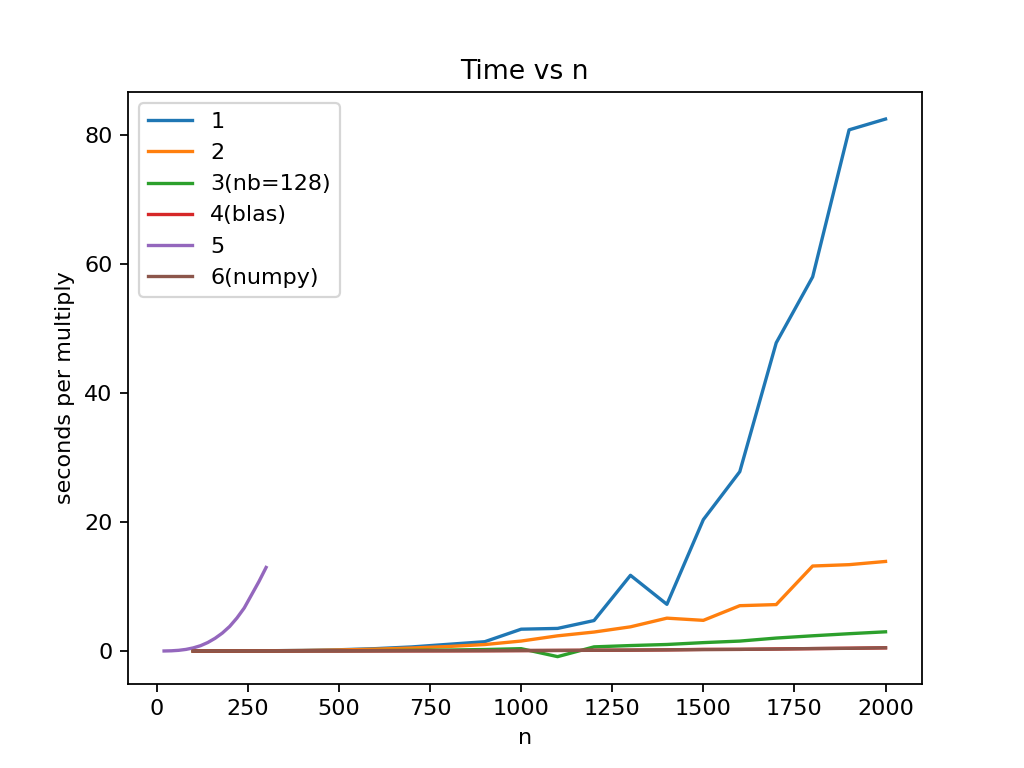
\includegraphics[width=0.82\linewidth]{plots/time_vs_n.png}
		\caption{Time per multiplication vs matrix size $n$.}
		\label{fig:time}
	\end{figure}
	
	\begin{figure}[H]
		\centering
		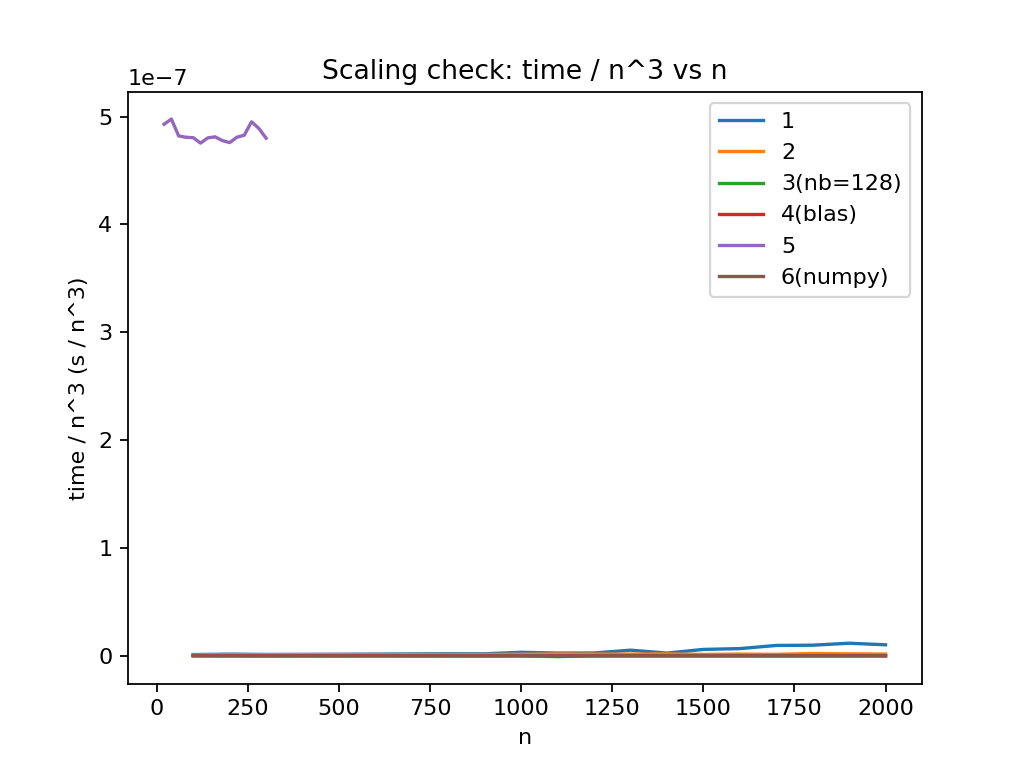
\includegraphics[width=0.82\linewidth]{plots/time_over_n3.png}
		\caption{Scaling check: $t/n^3$ vs $n$ (approximately flat indicates $O(n^3)$).}
		\label{fig:scaling}
	\end{figure}
	
	\begin{figure}[H]
		\centering
		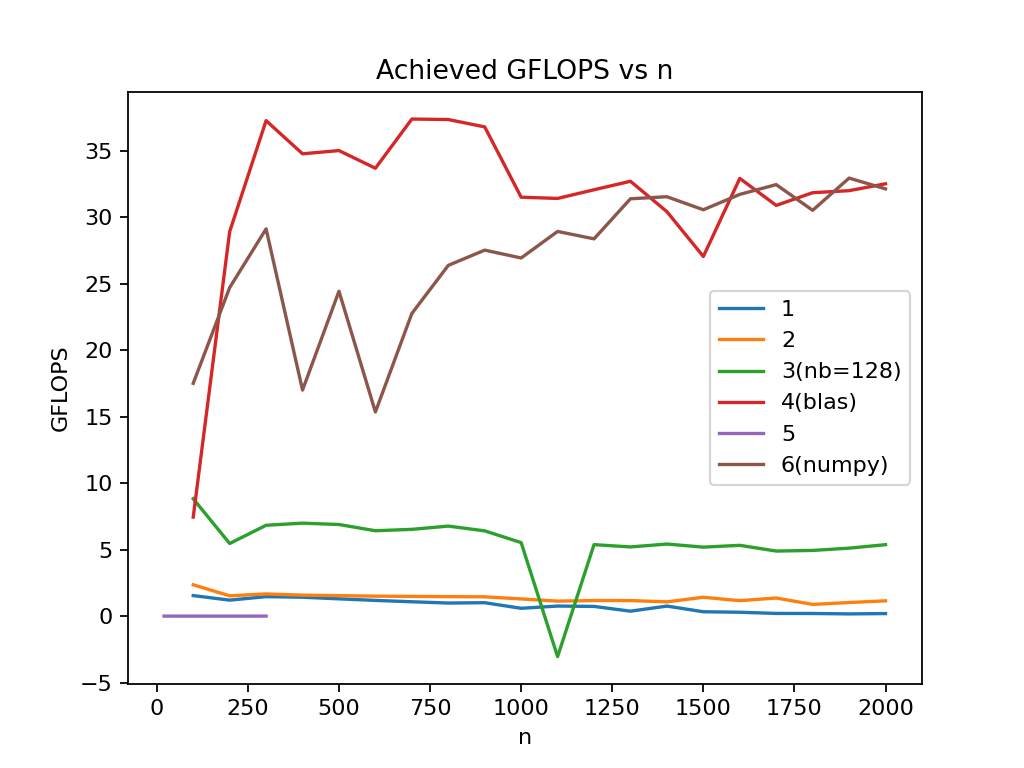
\includegraphics[width=0.82\linewidth]{plots/gflops_vs_n.png}
		\caption{Achieved GFLOPS vs $n$.}
		\label{fig:gflops}
	\end{figure}
	
	\begin{table}[H]
		\centering
		\caption{Sample timings and throughput for selected matrix sizes.}
		\begin{tabular}{llrrr}
			\toprule
			Language & Method & $n$ & Time (s) & GFLOPS \\
			\midrule
			C++ & 1 (naive)        & 200  & 0.00947  & 1.69 \\
			& 2 (transpose)    & 200  & 0.00804  & 1.99 \\
			& 3 (blocked,128)  & 200  & 0.00193  & 8.28 \\
			& 4 (BLAS)         & 200  & 0.00063  & 25.45 \\
			\midrule
			C++ & 1 (naive)        & 1000 & 2.689    & 0.74 \\
			& 2 (transpose)    & 1000 & 1.308    & 1.53 \\
			& 3 (blocked,128)  & 1000 & 0.268    & 7.45 \\
			& 4 (BLAS)         & 1000 & 0.04799  & 41.66 \\
			\midrule
			C++ & 1 (naive)        & 2000 & 81.22    & 0.20 \\
			& 2 (transpose)    & 2000 & 13.54    & 1.18 \\
			& 3 (blocked,128)  & 2000 & 3.356    & 4.77 \\
			& 4 (BLAS)         & 2000 & 0.5006   & 31.96 \\
			\midrule
			Python & 5 (loops)     & 200  & 3.807    & 0.004 \\
			& 6 (NumPy)     & 200  & 0.000646 & 24.70 \\
			Python & 5 (loops)     & 300  & 12.96    & 0.004 \\
			& 6 (NumPy)     & 1000 & 0.0742   & 26.93 \\
			& 6 (NumPy)     & 2000 & 0.498    & 32.12 \\
			\bottomrule
		\end{tabular}
		\label{tab:benchmarks}
	\end{table}
	
	
	\subsection{Observations}
	\textbf{Scaling.} Dividing runtime by $n^3$ gives nearly flat curves for C++ Methods~1--4 and NumPy, which is exactly what cubic complexity predicts. Small sizes wobble because fixed overheads, timer noise, and low arithmetic intensity dominate.  
	
	\textbf{Absolute time.} The plain triple loop (Method~1) explodes in cost and is unusable past $n \approx 1800$. Adding a transpose (Method~2) helps, but not enough to make it competitive. Blocking (Method~3) cuts times dramatically, and the BLAS routine (Method~4) wins outright across the board.  
	
	\textbf{Throughput.} DGEMM sustains about 30--37~GFLOPS on this CPU, with NumPy trailing just behind since it calls BLAS under the hood. The blocked kernel lands in the 5--9~GFLOPS range, though it stumbles around $n \approx 1100$ (likely cache or TLB oddities). Methods~1--2 limp along at 0.5--2.5~GFLOPS, bottlenecked by memory access.  
	
	\textbf{Cache and tiling.} The jump from Method~2 to Method~3 shows why tiling matters. Cutting the working set to $n_b \times n_b$ tiles keeps data in cache and lets each load do more useful work. With 512~KB L2, $n_b=128$ is a sensible choice; testing nearby sizes could squeeze out a bit more speed.  
	
	
	\textbf{Block size} Picking the block size $n_b$ was basically a game of fitting three blocks (A, B, and C) into L2 cache without blowing it up. With 512~KB available, $n_b=128$ made sense because the working set is about 0.39~MB, which sits comfortably in cache. The performance dip around $n \approx 1100$ shows that hardware is never perfectly predictable, but overall the choice was reasonable. Achieved performance of 30–37~GFLOPS for BLAS is about 70--85\% of the theoretical single-core peak ($\sim 43$~GFLOPS at 2.7~GHz with AVX2). For a laptop CPU running under WSL, that’s pretty respectable.
	
	\section{Discussion}
	The experiments highlight how strongly memory access patterns shape performance in dense $AB$. 
	Adding a transpose (Method~2) improves locality compared to the naive loop, but the working set is still too large to be efficient. 
	Tiling (Method~3) reduces the active footprint so that A, B, and C blocks are reused in cache, boosting arithmetic intensity and closing much of the gap to BLAS. 
	The optimized library routine (Method~4) goes further with data packing, prefetching, vector-aware micro-kernels, and loop unrolling, which is why it consistently beats my handwritten code. 
	On the Python side, raw loops (Method~5) are hopelessly slow, while NumPy (Method~6) essentially matches BLAS since it delegates everything to the same routines under the hood.  

	
	\section{Reproducibility}
	To reproduce:
	\begin{enumerate}
		\item Build with \verb|make| (OpenBLAS linked).
		\item \verb|source env_single_thread.sh|
		\item Run C++ and Python commands as listed above.
		\item Generate plots via \verb|scripts/plot_results.py|.
	\end{enumerate}
	
	\section{Conclusion}
	Raw python performed horribly. Standard textbook algorithm on C++ works faster than python simply by the virtue of being compiled and optimized. On my system, the block method works reasonably well, almost as well as Numpy or BLAS. NumPy achieves slightly worse performance by invoking BLAS under the hood. The data follow the expected $O(n^3)$ trend with overhead-driven deviations at small sizes. The best result is of course from BLAS because some underpaid Chinese PhD figured all out and optimized everything in assembly a long time ago.
	
	\section*{Acknowledgments}
	I credit Youtube and Chatgpt for the help.
	
	\section*{Honor Statement}
	\honor
	
	% Print bibliography only if a .bib exists
	\IfFileExists{references.bib}{\printbibliography}{}
	
\end{document}
